\documentclass[main.tex]{subfiles}
\section{2 point Boundary Value Problems}
2-point Boundary Value Problems (BVP) represent a special case of differential equations where the solution is limited by a pair of constraints at both ends of the interval. Hence, the task consists of finding the solution that apart from solving the differential equation satisfies the boundary conditions.

In the linear case, a numerical approximation to the  solution to these problems can be obtained solving a linear system. However, for nonlinear differential equations the solution is not straightforward and an iterative process is needed. In this exercise, we shall study different methods for solving nonlinear BVPs by applying them to the following differential equation:

\begin{equation}
\begin{aligned}
\epsilon u(t)'' + u(t)(u(t)'-1) = 0 \qquad 0\leq t\leq 1 \\
u(0) = \alpha \qquad u'(1) = \beta
\end{aligned}
\label{eq:problem1}
\end{equation}

\subsection{Newton's method}

If the independent variable $t$ is discretized and the second derivative in equation \ref{eq:problem1} is replaced by the centered difference method, an approximation to the solution at a series of equidistant points can be found solving the following scheme:

\begin{equation}
\begin{aligned}
\epsilon\left(\frac{u_{i-1} - 2 u_i + u_{i+1}}{h^2}\right) + u_i\left(\frac{u_{i+1} - u_{i-1}}{2 h} - 1\right) = 0 \\
u(0) = \alpha \qquad u(1) = \beta \\
\end{aligned}
\label{scheme}
\end{equation}

Where $i = 1,2, ..., m$ and $h$ is the distance between points in the interval.

The centered approximation comes from a Taylor series expansion truncated to the second term. We can show that the approximation is second-order accurate by computing the local error:

\begin{multline}
\tau_i = \epsilon\left(\frac{u(t_{i-1}) - 2 u(t_i) + u(t_{i+1})}{h^2}\right) + u_i\left(\frac{u(t_{i+1}) - u(t_{i-1})}{2 h} - 1\right) - \\
u(t_i)'' - u(t_i)(u(t_i)'-1)
\end{multline}

The above expression is just the difference between the given differential equation and its finite difference approximation. By applying the Taylor series expansion to the first two terms:

\begin{multline}
\tau_i = \epsilon\left(u''(t_i)+\frac{1}{12}h^2u'''(t_i)+O(h^4)\right) + u(t_i) \left(u'(t_i)+\frac{1}{6}h^2 u'''(t_i) + O(h^5)- 1 \right) -
\\ u(t_i)'' - u(t_i)(u(t_i)'-1) 
\end{multline}


\begin{equation}
\tau_i = \frac{1}{12}h^2u'''(t_i)+O(h^4) + u(t_i)(\frac{1}{6}h^2 u'''(t_i) + O(h^5))
\label{eq:localerror}
\end{equation}

The dominant term in equation \ref{eq:localerror} is then dependent of $h^2$ and thus we can conclude that the local truncation error is order $O(h^2)$.

Equation \ref{eq:scheme} can be expressed as a nonlinear system of the form:

\begin{equation}
G(U) = 0
\label{eq:scheme}
\end{equation}

And its roots can be obtained using Newton's method.

\begin{equation}
U^{[k+1]} = U^{[k]} + J(U^{[k]})^{-1} G(U^{[k]})
\label{eq:newtons}
\end{equation}

Where $U^{[k]}$ is a vector containing a discrete approximation to the solution after $k$ iterations and $J(U^{[k]})$ is the Jacobian matrix of the system, which in our case:


\begin{equation}
J(U) = 
\begin{cases}
\frac{\epsilon}{h^2} - \frac{u_i}{2 h} \qquad j = i - 1 \\
-\frac{2 \epsilon}{h^2} - \frac{u_{i+1}-u_{i-1}}{2 h}-1 \qquad  j = i \\
\frac{\epsilon}{h^2} + \frac{u_i}{2 h} \qquad j = i - 1 \\
\end{cases}
\end{equation}
 
Our implementation of the Newton's method consist of two functions: FunJac, which builds the vector $G$ and the tridiagonal matrix $J$ and NewtonsMethod, which updates the solution applying \ref{eq:newtons} until the tolerance is satisfied or the number of iterations is greater than the threshold.

The convergence and accuracy of the method depend on the proximity of the initial guess to the real solution. An approximation to the solution is given by equation 2.105 in LeVeque. Since an arbitrary choice might lead to non-convergence we have used this approximation as the initial value. \hl{It is shown in section 2.16.3 in Randall Leveque that the method is stable if the inverse of the Jacobian matrix is bounded}. Figure \ref{fig:newtons} shows the initial guess along with the solution returned by the Newton's method for 50 grid points.


\begin{figure}[H]
    \centering
    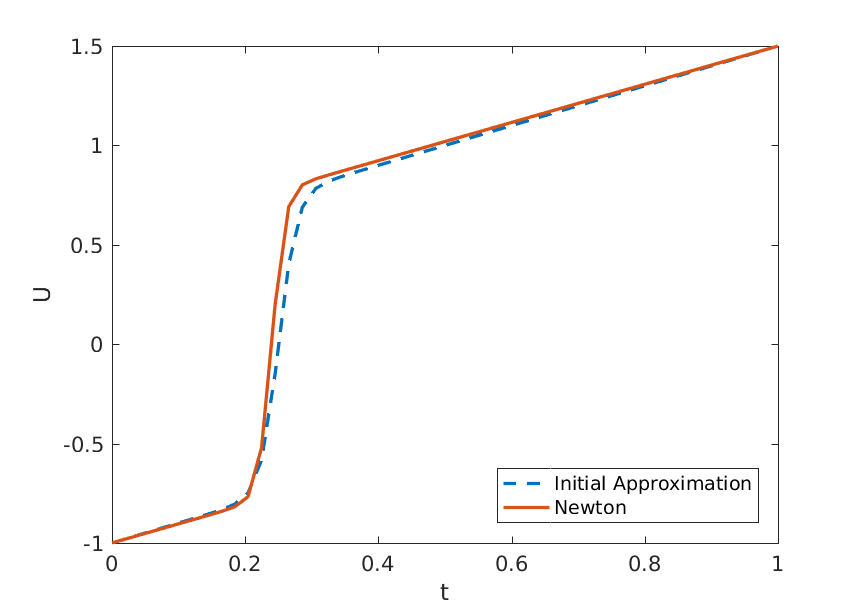
\includegraphics[width=\textwidth]{../Figures/newtons}
    \caption{Initial approximation and solution to the BVP using Newton's method for 50 grid points}
    \label{fig:newtons}
\end{figure}

The solution to \ref{eq:problem1} has also been computed using bvp4c function in MATLAB. Figure \ref{fig:sol} shows a comparative of the results obtained using Newton's method and bvp4c setting the tolerance equal to $0.01$ and 33 grid points.

\begin{figure}[H]
    \centering
    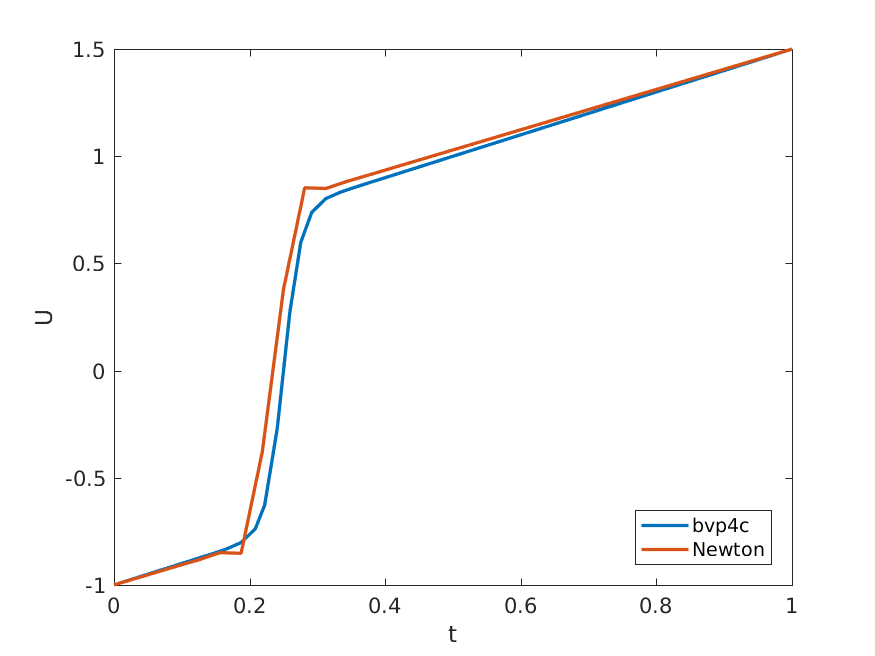
\includegraphics[width=\textwidth]{../Figures/sol}
    \caption{Initial approximation and solution to the BVP using Newton's method and bvp4c with 33 grid points}
    \label{fig:sol}
\end{figure}

Finally a more accurate approximation has been obtained setting the tolerance of bvp4c to $10^{-10}$. A section of the solution is shown in figure \ref{fig:sol2} along with the Newton's method solution now for $100$ grid points. The region shown in the graph corresponds to a layer where the solution changes rapidly. It is easy to see that Newton's method lies further from the true solution in this region. The number of points required to obtain a more accurate solution is greater than anywhere else due to this sudden variation. Hence, better results could be obtained using a non-uniform grid. The solution would be more finely discretized in the mentioned region and thus any rapid change could be easily controlled. 


\begin{figure}[H]
    \centering
    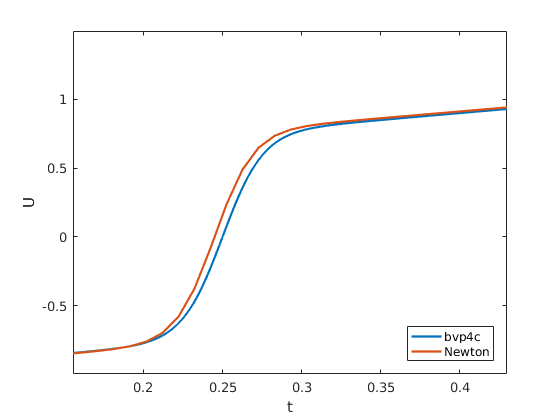
\includegraphics[width=\textwidth]{../Figures/sol2}
    \caption{Section of the solution to the BVP using Newton's method with 100 grid points and bvp4c for a tolerance of $10^{-10}$}
    \label{fig:sol2}
\end{figure}

\subsection{Single shooting}

One could also write the BVP in equation \ref{eq:problem1} as an initial value problem (IVP) of the form:

\begin{equation}
\begin{aligned}
\epsilon\left(\frac{u_{i-1} - 2 u_i + u_{i+1}}{h^2}\right) + u_i\left(\frac{u_{i+1} - u_{i-1}}{2 h} - 1\right) \\
u(0) = \alpha \qquad u'(0) = \sigma \\
\end{aligned}
\label{eq:ivp}
\end{equation}

Note that a new variable $\sigma$ has been included whose value must be chosen so that the second constraint in \ref{eq:problem1} is satisfied:

\begin{equation}
r(\sigma) = U(1,\sigma) - \beta = 0
\label{eq:roots}
\end{equation}

An approximation to the solution of the IVP can be computed in MATLAB using the function ode45. The naive way to tackle the problem would be to try different values of $\sigma$ and choose the one that yields the closest solution to the boundary constraint. However, the use of a numerical algorithm to find the root of \ref{eq:roots} would be computationally more convenient.

As a first approach we implemented the bisection method. Given two values of $\sigma$ for which equation \ref{eq:roots} has opposite sign we know that the solution will lie within the interval described by these two points. Consequently the solution is found by progressively reducing the interval until its size is below a tolerance. Although the algorithm will converge no matter the size of the interval, the problem now is translated into obtaining the two initial points. Moreover, the method presents a poor linear rate of convergence.

\begin{figure}[H]
    \centering
    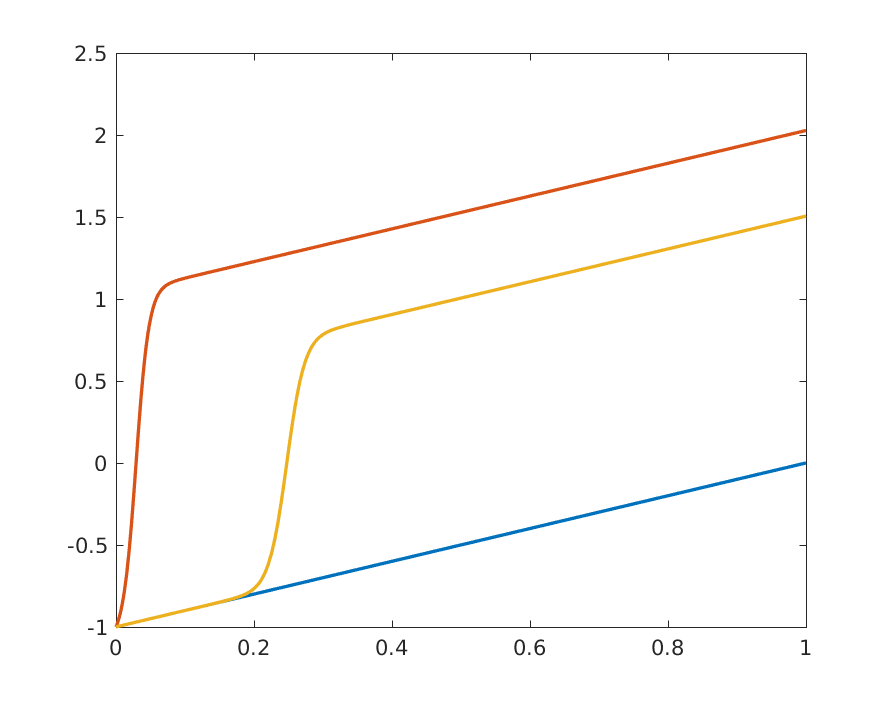
\includegraphics[width=\textwidth]{../Figures/bisection}
    \caption{Solution to the IVP using the bisection method. $U_a$ and $U_b$ are the two initial guess of opposite sign while $U_c$ is the solution that verifies the second boundary constraint}
    \label{fig:bisection}
\end{figure}

Figure \ref{fig:bisection} shows the solution obtained $U_c$ applying the bisection method along with the two initial guesses $U_a$ and $U_b$, of opposite sign with respect to the boundary constraint. We see that after a certain number of iterations the algorithm is able to hit the second constraint.

A more efficient algorithm can be obtained applying Newton's method. For that, we would like to have an expression for the first partial derivative of \ref{eq:roots} with respect to $\sigma$ so that the value of $\sigma$ can be updated in every iteration.

Since $\beta$ in \ref{eq:roots} is a constant we can write:

\begin{equation}
\frac{\partial r(\sigma)}{\partial \sigma} =  \frac{\partial u(1,\sigma)}{\partial \sigma}
\end{equation}

taking the partial derivative with respect to $\sigma$ in \ref{eq:ivp}:

\begin{equation}
\begin{aligned}
\frac{\partial u''}{\partial \sigma} =  \frac{-u'+1}{\epsilon} \frac{\partial u}{\partial \sigma} - \frac{u}{\sigma} \frac{\partial u'}{\partial \sigma} \\ 
\frac{\partial u(0)}{\partial \sigma} = 0 \qquad \frac{\partial u'(0)}{\partial \sigma} = 1  
\end{aligned}
\end{equation}

and since this is also an IVP it can be solved together with \ref{eq:ivp} as a single differential equation. As we mentioned before, Newton's method requires a suitable initial guess to converge. We experienced in this case that the algorithm is unable to converge for small values of $\epsilon$ in such cases, the bisection method should be applied. Figure \ref{fig:usigma} shows the solution at the end of the interval for a series of $\sigma$ values. Although a more detailed reason for the non-convergence of the method is given in the next section, it easy to see that the function is close to be non-differentiable in a neighborhood of $\sigma$ optima.

\begin{figure}[H]
    \centering
    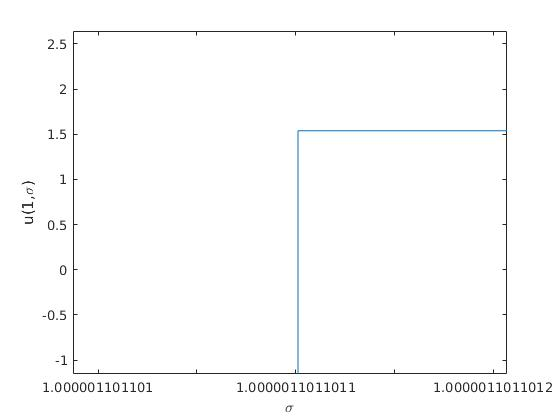
\includegraphics[width=\textwidth]{../Figures/usigma}
    \caption{Solution to the IVP at the last point of the interval for a series of $\sigma$ values close to the optima with $\epsilon = 0.01$}
    \label{fig:usigma}
\end{figure}



The rate of convergence of both algorithms has been plotted and can be seen in figure \ref{fig:rate}. The graph shows that for $\epsilon$ sufficiently large Newton's method converges quadratically.

\begin{figure}[H]
    \centering
    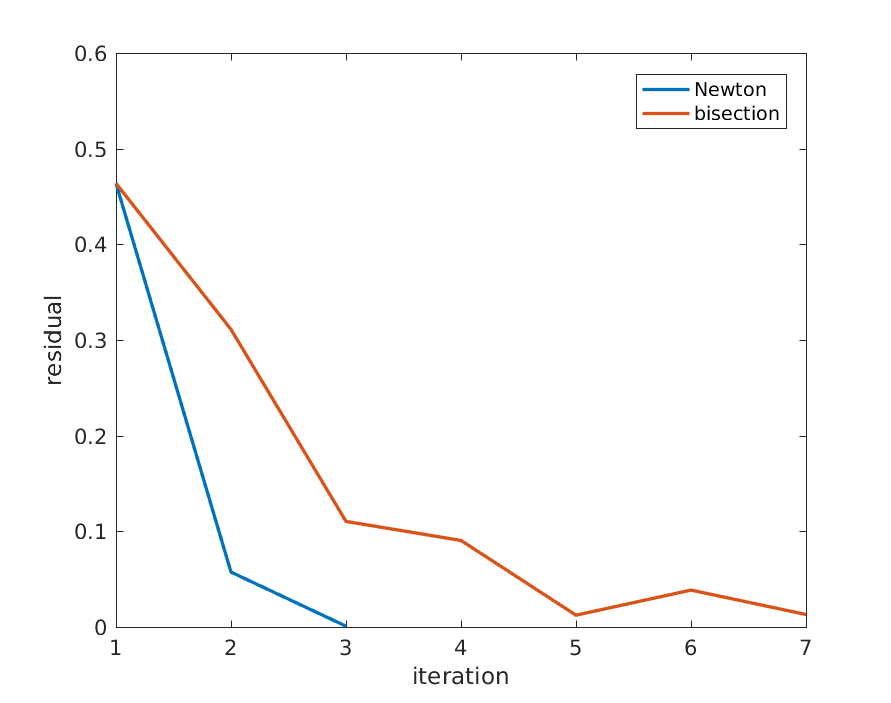
\includegraphics[width=\textwidth]{../Figures/rate}
    \caption{Newton and bisection algorithm rate of convergence for $\epsilon = 0.8$}
    \label{fig:rate}
\end{figure}


Finally the secant method is a variation of the Newton's algorithm where the derivative is approximated by finite difference so that there is no need for solving an extra differential equation. The code for all three algorithms is collected in the appendix. Besides, some information about the three methods performance is shown in table \ref{tab:shooting}.

\begin{table}
\centering
\begin{tabular}{c|lll} 
 \hline \hline
Method & Iterations & CPU-time  & \\ \hline 
Bisection & 8  & 0.0054 & \\ 
Newton & 3 & 0.0022 &  \\
Secant & 3 & 0.0036 &  \\
\hline \hline 
\end{tabular}
\caption{Number of iterations and CPU-time of all three algorithms with $\epsilon = 0.8$}
\label{tab:shooting}
\end{table}

\subsection{Sensitivity analysis and non-convergence}

In order to find an approximation to the partial derivative of the solution with respect to $\sigma$ we can either solve equation \ref{eq:ivp2} or apply the finite difference method. In both cases we see that for small values of $\epsilon$ the solution becomes very sensible to small variations of $\sigma$ (table \ref{tab:sensitivities}). On the other hand, as we saw in figure \ref{fig:usigma} equation \ref{eq:roots} was close to be non-smooth (non-differentiable) in a neighborhood of the solution. That is the reason why neither Newton's method nor the secant algorithm are able to converge even for initial guesses close to the true solution. 


\begin{table}
\centering
\begin{tabular}{c|lll} 
 \hline \hline
$\epsilon$ & $S_\sigma$  & \\ \hline 
0.01 & 1.0299$\times10^5$ &  \\
0.05 & 0.5791 &  \\
0.1 & 0.3620 &  \\
0.5 & 0.7110 &  \\
\hline \hline 
\end{tabular}
\caption{Number of iterations and CPU-time of all three algorithms with $\epsilon = 0.8$}
\label{tab:shooting}
\end{table}

If the initial value lies where the slope in figure \ref{fig:usigma} is almost 0 the method takes a very large step in the first update and the algorithm is unable to find the way back. If on the other hand, the initial value fells in a region where the curve is very steep, the step size in every iteration will be very small and the algorithm will never converge.

A way around would be to include an extra parameter that controls the step size every time $\sigma$ is updated. However, in this case the number of iterations increases dramatically for small values of $\epsilon$. Thus, it might be advisable to use an algorithm that does not require partial derivatives, such as the bisection method. Applying the bisection method with $\epsilon = 0.01$ the algorithm converges after $24$ iterations.
